\section{Типы данных – простые и составные. Агрегирование данных}

\subsection{Типы данных – простые и составные}

\newcommand{\minline}[1]{\mverb{#1}}

\begin{figure}[H]
    \centering
    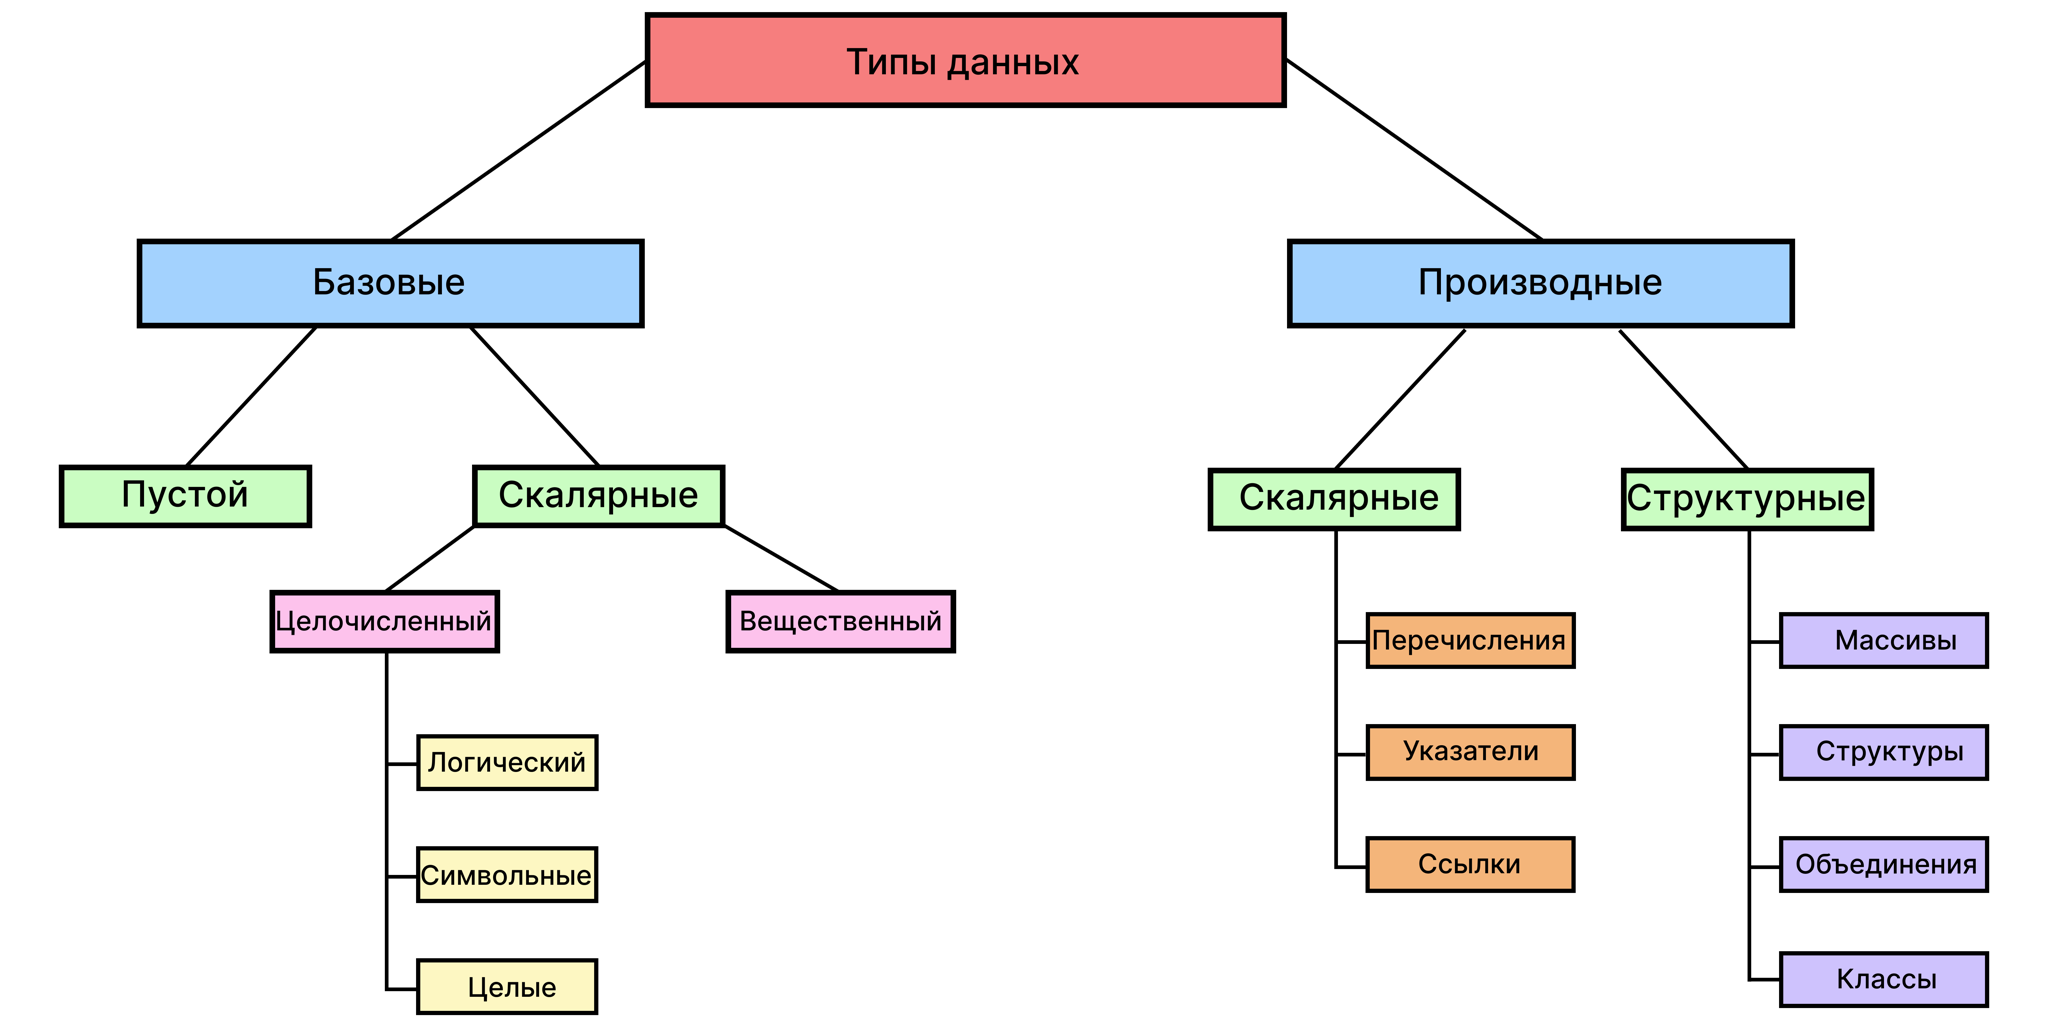
\includegraphics[width=\textwidth]{../semester-1/res/сpp-types.png}
    \caption{Типы данных C++}
\end{figure}

Типы данных языка C++ делятся на простые (базовые) и составные (производные).

\vspace{\baselineskip}

В категории базовых типов выделяют

\begin{enumerate}
    \item
          Пустой тип (он же \texttt{void} в \textbf{С++}).

          Нет и не может быть объектов этого типа. Используется в отклонении
          (англ. \emph{discard}) результата вычисления (прим.
          \minline{(void)GetAnswerToTheUniverse();}) и в функциях, не
          возвращающих значений.
    \item
          Скалярные типы

          \begin{itemize}
              \item
                    Целочисленные типы: логический (\texttt{bool} в \textbf{С++}),
                    символьный (\texttt{char}, \texttt{wchar\_t}, \texttt{char32\_t},
                    \ldots), целый (\texttt{int}, \texttt{short}, \ldots)
              \item
                    Вещественный тип
          \end{itemize}
\end{enumerate}

В категории производных типов выделяют

\begin{enumerate}
    \item
          Скалярные типы

          Перечисления (\texttt{enum}), указатели (\texttt{<тип> *}), ссылки (\texttt{<тип> \&}).
    \item
          Структурные типы

          Массивы (\texttt{<тип>[<размер>]} (статический)), структуры (\texttt{struct}), объединения (\texttt{union}), классы (\texttt{class}).
\end{enumerate}

Отдельно рассмотрим целочисленные и вещественные типы данных в
\textbf{С++}.

\subsubsection{Целочисленные типы}

Стоит отметить, что размеры конкретных типов зависят от платформы.
Стандарт \textbf{С++} дает ограниченные гарантии на их размер. Также к
ключевым словам типов (\texttt{int}, \texttt{short}, \texttt{long})
могут добавляться квалификаторы \texttt{signed} (определяет знаковость)
и \texttt{unsigned} (определяет беззнаковость). Возможна и комбинация
ключевых слов типов: \texttt{unsigned\ long\ long\ int}.

\begin{scriptsize}
    \begin{longtable}[]{@{}
        >{\raggedright\arraybackslash}p{(\columnwidth - 12\tabcolsep) * \real{0.2418}}
        >{\raggedright\arraybackslash}p{(\columnwidth - 12\tabcolsep) * \real{0.2413}}
        >{\raggedright\arraybackslash}p{(\columnwidth - 12\tabcolsep) * \real{0.1139}}
        >{\raggedright\arraybackslash}p{(\columnwidth - 12\tabcolsep) * \real{0.0759}}
        >{\raggedright\arraybackslash}p{(\columnwidth - 12\tabcolsep) * \real{0.0844}}
        >{\raggedright\arraybackslash}p{(\columnwidth - 12\tabcolsep) * \real{0.1181}}
        >{\raggedright\arraybackslash}p{(\columnwidth - 12\tabcolsep) * \real{0.1646}}@{}}
        \toprule\noalign{}
        \begin{minipage}[b]{\linewidth}\raggedright
            Тип
        \end{minipage}                                 & \begin{minipage}[b]{\linewidth}\raggedright
                                                             Эквивалентен
                                                         \end{minipage} & \begin{minipage}[b]{\linewidth}\raggedright
                                                                              Пояснение
                                                                          \end{minipage} & \begin{minipage}[b]{\linewidth}\raggedright
                                                                                               Минимальный размер
                                                                                           \end{minipage} & \begin{minipage}[b]{\linewidth}\raggedright
                                                                                                                Размер на \emph{x86-64}
                                                                                                            \end{minipage} & \begin{minipage}[b]{\linewidth}\raggedright
                                                                                                                                 Диапазон значений (\emph{x86-64})
                                                                                                                             \end{minipage} & \begin{minipage}[b]{\linewidth}\raggedright
                                                                                                                                                  Примечание
                                                                                                                                              \end{minipage}                                                   \\
        \midrule\noalign{}
        \endhead
        \bottomrule\noalign{}
        \endlastfoot
        \texttt{signed\ char}                                                       & \texttt{signed\ char}                       & Символьный тип                              & 8 бит                                       &
        8 бит                                                                       & -128 до 127                                 &                                                                                                        \\
        \hline \texttt{unsigned\ char}                                              & \texttt{unsigned\ char}                     & Символьный тип                              & 8
        бит                                                                         & 8 бит                                       & 0 до 255                                    &                                                          \\
        \hline \texttt{char8\_t}                                                    & \texttt{char8\_t}                           & Символьный тип для UTF-8                    & 8 бит
                                                                                    & 8 бит                                       & 0 до 255                                    & С \textbf{С++20}                                         \\
        \hline \texttt{wchar\_t}                                                    & \texttt{wchar\_t}                           & Длинный символьный тип                      & -                                           &
        зависит от платформы                                                        & зависит от платформы                        & На Unix/Linux - 32\par На
        Windows - 16                                                                                                                                                                                                                       \\
        \hline \texttt{char16\_t}                                                   & \texttt{char16\_t}                          & Символьный тип для UTF-16                   & 16
        бит                                                                         & 16 бит                                      & 0 до 65535                                  &                                                          \\
        \hline \texttt{char32\_t}                                                   & \texttt{char32\_t}                          & Символьный тип для UTF-32                   & 32
        бит                                                                         & 32 бит                                      & 0 до 1114111 (\emph{0x10ffff})              & Ограничение Unicode                                      \\
        \hline \texttt{short}\par \texttt{short\ int}\par \texttt{signed\ short}\par \texttt{signed\ short\ int}
                                                                                    & \texttt{short\ int}                         & Целый тип, не больший \texttt{int}          & 16 бит                                      & 16
        бит                                                                         & −32768 до 32767                             &                                                                                                        \\
        \hline \texttt{unsigned\ short}\par \texttt{unsigned\ short\ int}           &
        \texttt{unsigned\ short\ int}                                               & Беззнаковый \texttt{short}                  & 16 бит                                      & 16
        бит                                                                         & 0 до 65535                                  &                                                                                                        \\
        \hline \texttt{int}\par \texttt{signed}\par \texttt{signed\ int}            & \texttt{int}                                &
        Основной целый тип                                                          & 16 бит                                      & 32 бит                                      & \(-2^{31}\) до \(2^{31}-1\)                 &            \\
        \hline \texttt{unsigned}\par \texttt{unsigned\ int}                         & \texttt{unsigned\ int}                      &
        Беззнаковый \texttt{int}                                                    & 16 бит                                      & 32 бит                                      & 0 до \(2^{32}-1\)                           &            \\
        \hline \texttt{long}\par \texttt{long\ int}\par \texttt{signed\ long}\par \texttt{signed\ long\ int}
                                                                                    & \texttt{long\ int}                          & \emph{Длинное} целое                        & 32 бит                                      & зависит от
        платформы                                                                   & зависит от платформы                        & На Unix/Linux - 64\par Windows API - 32                                                                \\
        \hline \texttt{unsigned\ long}\par \texttt{unsigned\ long\ int}             &
        \texttt{unsigned\ long\ int}                                                & Беззнаковый \texttt{long}                   & 32 бит                                      &
        зависит от платформы                                                        & зависит от платформы                        & На Unix/Linux - 64\par Windows
        API - 32                                                                                                                                                                                                                           \\
        \hline \texttt{long\ long}\par \texttt{long\ long\ int}\par \texttt{signed\ long\ long}\par \texttt{signed\ long\ long\ int}
                                                                                    & \texttt{long\ long\ int}                    & \emph{Дважды длинное} целое                 & 64 бит                                      & 64
        бит                                                                         & \(-2^{63}\) до \(2^{63}-1\)                 &                                                                                                        \\
        \hline \texttt{unsigned\ long\ long}\par \texttt{unsigned\ long\ long\ int} &
        \texttt{unsigned\ long\ long\ int}                                          & Беззнаковый \texttt{long\ long}             &
        64 бит                                                                      & 64 бит                                      & 0 до \(2^{64}-1\)                           &                                                          \\
    \end{longtable}
\end{scriptsize}

\begin{quote}
    Тип \texttt{char} занимает по крайней мере 8 бит и ведет себя так же,
    как и \texttt{signed\ char} или \texttt{unsigned\ char}, но является
    отдельным типом. При этом конкретная знаковость зависит от платформы и
    настроек компилятора. На \emph{x86} он обычно знаковый, на \emph{arm} -
    обычно беззнаковый.
\end{quote}

\begin{quote}
    Логический тип \texttt{bool} занимает по крайней мере 8 бит и хранит
    лишь два значения - \texttt{true} или \texttt{false}.
\end{quote}

Типы в \textbf{С++} формируют иерархию по размеру:
\begin{minted}{C++}
1 == sizeof(char) <= sizeof(short) <= sizeof(int) <= sizeof(long) <= sizeof(long long)
\end{minted}

Однако стандарт гарантирует лишь минимальное количество бит типов. В
частности возможная абсурдная ситуация, когда на платформе один байт\footnote{Под \textit{байтом} в этом контексте понимается минимально адресуемый объем
    памяти. Это не обязательно `байт' в значении \textit{объем информации}.}
занимает 64 бит и
\begin{minted}{C++}
sizeof(char) == sizeof(short) == sizeof(int) == sizeof(long) == sizeof(long long) == 1
\end{minted}

Количество бит, которое занимает тип \texttt{char} можно проверить
макросом \texttt{CHAR\_BIT}; впрочем, практически все современные
системы имеют байт\footnotemark[\value{footnote}] равным 8 бит.

\subsubsection{Вещественные типы}

Стандарт \textbf{С++} определяет следующие типы с плавающей точкой
\begin{enumerate}
    \item \minline{float} - вещественный тип одинарной точности. Обычно
          \textbf{IEEE 754} \emph{binary32}.
    \item \minline{double} - вещественный тип
          двойной точности. Обычно \textbf{IEEE 754} \emph{binary64}.
    \item \minline{long double} - вещественный тип повышенной точности.
          \begin{quote}
              На разных платформах может быть типом четверной точности (\textbf{IEEE 754} \textit{binary128}), 80-битным \textit{x87-80 extended precision format} на \textit{x86}, быть эквивалентным `double` или реализован каким-либо другим образом.
          \end{quote}
\end{enumerate}

\subsubsection{Перечисления}

\textbf{Перечисление} -- это определяемый пользователем тип, состоящий из набора именованных \underline{целочисленных констант}, которые называются \textit{перечислителями}.

\vspace{\baselineskip}

Перечисление имеет следующую форму:
\begin{minted}{C++}
enum class имя_перечисления { константа_1, константа_2, ... константа_N };
\end{minted}

Каждой константе сопоставляется некоторое числовое значение. По умолчанию первая константа получает в качестве значения 0, а остальные увеличиваются на единицу.

\vspace{\baselineskip}

Определим простейшее перечесление:
\begin{minted}{C++}
enum class Day {Monday, Tuesday, Wednesday, Thursday, Friday, Saturday, Sunday};
\end{minted}

После создания перечисления мы можем определить его переменную и присвоить ей одну из констант:

\begin{minted}{C++}
Day today {Day::Thursday};
// или Day today = Day::Thursday;
\end{minted}

Также мы можем управлять установкой значений в перечислении. Так, мы можем задать начальное значение для одной контанты, тогда у последуюших констант значение увеличивается на единицу:
\begin{minted}{C++}
enum class Day {Monday, Tuesday = 3, Wednesday, Thursday, Friday, Saturday, 
                Sunday};
\end{minted}

Стоит учитывать, что константы перечисления должны представлять целочисленные константы. Однако мы можем выбрать другой целочисленный тип, например, \texttt{char}:

\begin{minted}{C++}
enum class Operation: char {Add = '+', Subtract='-', Multiply='*'};
\end{minted}

Стоит отметить, что раньше в С++ использовалась другая форма перечислений, которые пришли из языка С и определяются без ключевого слова \texttt{class}. Такие перечисления еще называют \texttt{unscoped} (то есть не ограниченные ни какой областью видимостью). Естественно такие перечисления можно встретить в старых программах. Однако в виду того, что они потенциально могут привести к большему количеству ошибок, то в настоящее время такая форма все меньше и меньше используется.

\subsubsection{Указатели}

Указатель — это переменная, в которой хранится адрес памяти объекта. Указатели широко используются как в C, так и в C++ для трех основных целей:
\begin{itemize}
    \item для выделения новых объектов в куче,
    \item передача функций другим функциям
    \item для итерации элементов в массивах или других структурах данных.
\end{itemize}

Подробнее см. главу \ref{pointers_and_refs}.

\subsubsection{Ссылки}

В ссылке, как и в указателе, хранится адрес объекта, расположенного в другой области памяти. В отличие от указателя, ссылка после инициализации не может быть сделана, чтобы ссылаться на другой объект или задать значение \mverb{NULL}. Существует два типа ссылок: ссылки \textit{lvalue}, которые ссылаются на именованную переменную и ссылки \textit{rvalue}, которые ссылаются на временный объект. Оператор \mverb{&} обозначает ссылку \textit{lvalue}, а \mverb{&&} оператор обозначает либо ссылку rvalue, либо универсальную ссылку (\textit{rvalue} или \textit{lvalue}) в зависимости от контекста.

Подробнее см. главу \ref{pointers_and_refs}.

\subsubsection{Массивы}

Массив представляет собой последовательность объектов того же типа, которые занимают непрерывную область памяти. Традиционные массивы стилей C являются источником многих ошибок, но по-прежнему распространены, особенно в старых базах кода. В современном C++ настоятельно рекомендуется использовать \mverb{std::vector} или \mverb{std::array} вместо массивов стилей C.

Подробнее см. главу \ref{static_and_dynamic_data_structures}.

\subsubsection{Структуры}

\textbf{Структура} \label{def:struct} --- производный тип данных, который представляет какую-то определенную сущность.
Для определения структуры используется ключевое слово \verb|struct|:
\begin{minted}{C++}
struct ИмяСтруктуры {
  поля_структуры;
};
\end{minted}
Поля структуры --- это объявленные внутри структуры переменные, доступ к которым можно получать через объект структуры
с помощью оператора \verb|.| или через указатель на объект структуры через оператор \verb|->|.

В языке C, в отличие от C++, объявленная таким образом структура будет доступна под именем
\verb|struct ИмяСтруктуры| (в C++ --- просто \verb|ИмяСтруктуры|). Чтобы не писать слово
\verb|struct|, можно объявить псевдоним для типа структуры с помощью ключевого слова
\verb|typedef|. В C++ так тоже можно делать для обратной совместимости с Си. В C++
для полей структур можно задавать значения по умолчанию.

{\small В языке C++ во всех структурах неявно объявляется конструктор и деструктор по умолчанию
(если они не объявлены явно). Конструктор вызывается при объявлении (и/или инициализации) объекта
структуры (также при вызове оператора \verb|new|), а деструктор --- когда объект покидает
область видимости или вызывается оператор \verb|delete|.}

\subsubsection{Объединения}

\textbf{Объединение} --- группирование переменных, которые разделяют одну и ту же область памяти.

Объявление объединения (типа объединения или шаблона объединения) начинается с ключевого слова union.
\begin{minted}{C++}
union ИмяТипаОбъединения {
  Тип1 переменная_1;
  Тип2 переменная_2;
  ...
  ТипN переменная_n;
};
\end{minted}

Где \textbf{ИмяТипаОбъединения} --- непосредственно имя новосозданного объединения;

\textbf{переменная\_1, \dots, переменная\_n} --- имена переменных, которые являются полями объединения.
Эти переменные могут быть разных типов;

\textbf{Тип1, \dots, ТипN} --- типы полей объединения.

\paragraph{Размер объединения} равен размеру самого большого поля.

Объединение относится к определенному участку памяти, в котором может находиться объект одного из типов, которые есть в объединении. При попытке перезаписать данные другим типом новые данные записываются поверх старых, а для старых данных деструктор не вызывается. Поэтому в \verb|union| без дополнительных плясок с бубном нельзя поместить <<умный>> производный тип наподобие \verb|std::string|.

При обращении к полю объединения записанные в память данные будут
интерпретироваться как данные того типа, к которому относится переменная, к которой происходит обращение. Нетрудно догадаться, что обращение к неправильному типу может вызвать UB.

\subsubsection{Классы}

Кроме использования встроенных типов, таких как \mverb{int}, \mverb{double} и т.д., мы можем определять свои собственные типы или классы. \textbf{Класс} представляет составной тип, который может использовать другие типы.

Класс в C++ — это шаблон для создания объектов, который объединяет данные и функции, работающие с этими данными. Объявление класса позволяет описать не только данные представления объекта, но и аспекты использования таких данных:

\begin{itemize}
    \item список функций доступа к объектам
    \item правила наследования объектов производными классами
    \item различная степень инкапсуляции элементов класса
\end{itemize}

\begin{minted}{C++}
class Person 
{
public:
    std::string name;
    unsigned age;
    void print() 
    {
        std::cout << "Name: " << name << "\tAge: " << age << std::endl;
    }
};
\end{minted}

\subsection{Агрегирование данных}

Составные типы данных, также называемые сложными или агрегированными, задаются пользователем и могут включать в себя типы массивов, типы функций, типы классов (или структур), типы объединения, перечисления, ссылки и указатели на объекты.

\textbf{Агрегирование данных} - это процесс объединения нескольких переменных в одну структуру или класс

\section{Указатели и ссылки в языке С++. Семантика копирования и перемещения} \label{pointers_and_refs}

\subsection{Указатели}

Указатели представляют собой объекты, значением которых служат адреса других объектов (переменных, констант, указателей) или функций. Как и ссылки, указатели применяются для косвенного доступа к объекту. Однако в отличие от ссылок указатели обладают большими возможностями.

\vspace{\baselineskip}

\noindent Определение указателя:
\begin{minted}{C++}
тип_данных *название_указателя;
// либо тип_данных* название_указателя;
\end{minted}

Cтоит отметить что положение звездочки (\mverb{*}) не влияет на определение указателя: ее можно помещать ближе к типу данных, либо к имени переменной - оба определения будут равноценны.

Также стоит отметить, что размер значения указателя (хранимый адрес) не зависит от типа указателя. Он зависит от конкретной платформы. На 32-разрядных платформах размер адресов равен 4 байтам, а на 64-разрядных - 8 байтам.

С помощью операция \mverb{&} можно получить адрес некоторого объекта, например, адрес переменной. Затем этот адрес можно присвоить указателю.

\vspace{\baselineskip}

\noindent\underline{Пример}:
\begin{minted}{C++}
int num = 42;
int *pnum = &num; // взятие адреса переменной num
*num = 24; // разыменовывание указателя 
int temp = *num;
std::cout << temp << '\n'; // 24
\end{minted}

\subsubsection{Умные указатели}

\textbf{Smart pointers} или "интеллектуальные указатели" -- это объекты, которые имитируют стандартные указатели: они также содержат адрес (как правило, адрес выделенной динамической памяти), и их можно также использовать для обращения к объектам по этому адресу. Но главное их отличие от стандартных указателей состоит в том, что нам не надо беспокоиться об освобождении памяти с помощью операторов \mverb{delete} или \mverb{delete[]}. Вся выделенная память, используемая интеллектуальными указателями, будет освобождаться автоматически, когда она станет не нужна. Соответственно это означает, что мы не столкнемся с утечками памяти, не соответствием между выделениями и освобождениями памяти и болтающимися указателями. Таким образом, smart-указатели позволяют упростить и обезопасить управление памятью. Типы интеллектуальных указателей определены в модуле memory стандартной библиотеки языка С++ и доступны в пространстве имен \texttt{std}.

В C++11 появилось три типа умных указателей, все они определены в заголовке из Стандартной библиотеки:
\begin{itemize}
    \item \mverb{std::unique_ptr} — умный указатель, владеющий динамически выделенным ресурсом;
    \item \mverb{std::shared_ptr} — умный указатель, владеющий разделяемым динамически выделенным ресурсом. Несколько \mverb{std::shared_ptr} могут владеть одним и тем же ресурсом, и внутренний счетчик ведет их учет;
    \item \mverb{std::weak_ptr} — подобен \mverb{std::shared_ptr}, но не увеличивает счетчик.
\end{itemize}

Если вы хотите понять как работать с умными указателями на базовом уровне, рекомендую данную \href{https://habr.com/ru/companies/piter/articles/706866/}{статью на Habr}.

\subsection{l-value и r-value}

\begin{itemize}
    \item
          В языке C++, все переменные являются l-values, l-value, то есть они имеют свой собственный адрес в памяти. l от слова «left», так как только значения l-values могут быть использованы в качестве операнда в левой части операции присваивания(в противоположном случае, мы получим ошибку), а также в других контекстах, где требуется изменяемое значение.
    \item
          Противоположностью l-value является r-value. r-value - это выражение, которое имеет временное значение, которое не может быть использовано в качестве операнда в левой части операции присваивания. Например, число \mverb{42} или результат выражения \mverb{42 + х} являются r-values. Они не имеют адреса в памяти и не могут быть изменены. Обычно r-value используется в качестве операнда в правой части операции присваивания и других контекстах, где требуется неизменяемое значение.
    \item
          x-values (eXpiring values) - это категория значений, которая была введена в C++11 для представления объектов, которые находятся в конце своего жизненного цикла и могут быть перемещены в другой объект. Они представляют собой изменяемые r-values, но не имеют адреса в памяти. Примерами x-values могут быть объекты, которые были созданы с помощью функции \mverb{std::move()} или которые являются результатом выражения \mverb{std::move()};
\end{itemize}

\href{https://en.cppreference.com/w/cpp/language/value_category.html}{Cppreference - Value categories}

\subsection{Ссылки}

В C роль ссылок играют указатели, но работать с ними не очень удобно и в C++ появилась отдельная сущность — ссылка (reference). В C++11 ссылки получили дальнейшее развитие, появились rvalue-ссылки, универсальные (передаваемые) ссылки, которые играют ключевую роль в реализации семантики перемещения — одном из самых значительных нововведений C++11.

\begin{minted}{C++}
T x;
T &rx = x; // определение ссылки
T &rx2 = rx; // определение копии ссылки
\end{minted}

Инициализация ссылки обязательна, нулевые ссылки (ссылки на «ничто») не поддерживаются. Изменить переменную, на которую ссылается ссылка, невозможно. Таким образом, ссылка является константной сущностью, хотя формально ссылочный тип не является константным.

Собственных операций ссылка не поддерживает, все операторы, примененные к ссылке, на самом деле применяются к переменной, на которую она ссылается. Это касается и таких операторов, как \mverb{=} (присваивание), \mverb{&} (получение адреса), \mverb{sizeof}, \mverb{typeid}. Но вот спецификатор \mverb{decltype}, если его применить к ссылке, дает ссылочный тип.

Если T некоторый неконстантный и нессылочный тип или псевдоним, то можно определить ссылку на константу. Через ссылку на константу нельзя модифицировать объект, на которой она ссылается. Это означает, что для встроенных типов через такую ссылку запрещено присваивание, инкремент, декремент, а для пользовательских типов запрещен вызов неконстантных функций-членов.

\subsubsection*{Ссылки r-value}

В C++11 был добавлен новый тип ссылок - \textbf{ссылки r-value}, которые позволяют получать доступ к r-values и x-values. Они используются для реализации семантики перемещения и эффективной передачи аргументов функций. В то время как ссылка l-value создается с использованием одного амперсанда, ссылка r-value создается с использованием двойного амперсанда:

\begin{minted}{C++}
int &&rref = 42; // инициализация ссылки r-value литералом 42 (значение r-value)
\end{minted}

\href{https://habr.com/ru/articles/646005/}{Достаточно подробная статья о ссылках}

\subsection{Семантика копирования и перемещения}

\subsubsection{Конструктор и оператор копирования}

Конструктор копирования в C++ используется для создания копии объекта класса при инициализации. Оператор присваивания копированием (или «копирующее присваивание») используется для копирования одного объекта класса в другой существующий объект. По умолчанию компилятор автоматически предоставляет конструктор копирования и оператор присваивания копированием, если они не определены пользователем. Однако, эти автоматически сгенерированные функции выполняют только поверхностное копирование, что может приводить к проблемам у классов, работающих с динамической памятью. Для решения этих проблем необходимо переопределить конструктор копирования и оператор присваивания копированием, чтобы они выполняли глубокое копирование данных.

\begin{minted}{C++}
class T 
{
public:
    // ...
    T(const T &other) // конструктор копирования
    {
        // реализации копирования, например переприсвоение полей
    }
    // ...
    T& operator=(const T &other); // оператор копирования
    // ...
}
\end{minted}

\subsubsection{Конструктор и оператор перемещения}

В C++11 были добавлены две новые функции - конструктор перемещения и оператор присваивания перемещением - для работы с семантикой перемещения.В отличие от семантики копирования, которая заключается в создании копии объекта, целью семантики перемещения является перенос владения ресурсами из одного объекта в другой. Это более эффективный процесс, чем копирование, так как он не требует создания новых ресурсов и копирования данных. Особенно полезно использовать семантику перемещения для объектов, которые управляют большими блоками памяти или ресурсами, например, файловыми дескрипторами.

Конструктор перемещения и оператор присваивания перемещением определяются так же, как и конструктор и оператор присваивания копированием. Однако, вместо константной ссылки l-value, функции с перемещением принимают неконстантную ссылку r-value в качестве параметра.

\begin{minted}{C++}
class T 
{
public:
    // ...
    T(T &&other); // конструктор перемещения
    // ...
    T& operator=(T &&other); // оператор перемещения
    // ...
}
\end{minted}

Конструктор перемещения и оператор присваивания перемещением вызываются, когда аргументом для создания или присваивания является r-value. Чаще всего это будет литерал или временное значение, то есть временный объект.

В большинстве случаев конструктор перемещения и оператор присваивания перемещением не предоставляются по умолчанию. Однако, если это возможно, эти функции могут быть предоставлены по умолчанию, и в этом случае они будут выполнять то же самое, что и конструктор копирования и оператор присваивания копированием, то есть копирование, а не перемещение.

Если мы создаем объект или выполняем присваивание, где аргументом является r-value, то мы знаем, что это временный объект. Вместо копирования его ресурсов, что может быть затратно, мы можем просто переместить их в другой объект, который мы создаем или которому присваиваем текущий. Это безопасно, потому что временный объект будет уничтожен в конце выражения, поэтому мы можем быть уверены, что он никогда не будет повторно использован.

\section{Функции в языке С++. Понятие метода. Рекурсия}

\subsection{Функция}

Функции — это блоки кода, выполняющие определенные операции. Если требуется, функция может определять входные параметры, позволяющие вызывающим объектам передавать ей аргументы. При необходимости функция также может возвращать значение как выходное. Функции полезны для инкапсуляции основных операций в едином блоке, который может многократно использоваться. В идеальном случае имя этого блока должно четко описывать назначение функции.

\begin{minted}{C++}
тип имя_функции(параметры) // объявление функции
{              // 
    инструкции // определение функции
}              //
\end{minted}

Функция может вызываться из любого количества мест в программе. Значения, передаваемые функции, являются \textit{аргументами}, типы которых должны быть совместимы с типами параметров в определении функции.

\subsection{Метод}

Методы - это функции, объявление которых размещено внутри определения класса или структуры. В список переменных, доступных для метода, неявно попадают все поля структуры или класса, в котором он объявлен. Другими словами, в список областей видимости метода попадает область видимости структуры.

\begin{minted}{C++}
class T
{
private:
    int num;

public:
    T() { num = 42; }

    int getNum() { return num; } // метод, в данном случае геттер
}
\end{minted}

Существует несколько видов методов
\begin{itemize}
    \item обычные методы класса
    \item статический методы класса -- не зависят от экземпляра класса, то есть могут вызываться без него, но не имеют доступ к нестатичексим полям класса. \mverb{static}
    \item виртуальные методы -- это функция-член, которую предполагается переопределить в производных классах. \mverb{virtual}
    \item константные методы -- могут вызываться как для константных, так и для константных объектов, в них НЕ должны изменяться поля объекта. \mverb{const}
\end{itemize}

\subsection{Рекурсия}

\textbf{Рекурсивная функция} -- такая функция, которая вызывает саму себя.
Тривиальным примером рекурсивной функции может служить функция для вычисления чисел Фибоначчи, определяемых рекуррентным соотношением $f_n = f_{n-1} + f_{n-2} \quad (n \geq 3)$, причем $f_1 = f_2 = 1$:
\begin{minted}{C++}
long FibRecursion(long n) {
  if (n == 1 || n == 2) {
    return 1;
  }
  return FibRecursion(n - 1) + FibRecursion(n - 2);
}  
\end{minted}

Математически доказуемо, что любой рекурсивный алгоритм можно реализовать с помощью цикла и обратно: любой циклический алгоритм можно реализовать с помощью рекурсии.
\begin{minted}{C++}
long FibLoop(long n) {
  long f1 = 1;
  long f2 = 1;
  for (int i = 1; i <= n; ++i) {
    f1 += f2;
    std::swap(f1, f2);
  }
  return f2;
}
\end{minted}

Рекурсия используется во многих алгоритмах, например в сортировках Quicksort и Mergesort, в обходе графов (поиск в глубину).

Рекурсивные алгоритмы из-за накладных расходов на вызов функции обычно показывают худшую производительность чем циклические, несмотря на одинаковую
асимптотику. Кроме того, для работы рекурсивных алгоритмов необходимо поддерживать стек вызовов. Но размер стека ограничен, что накладывает ограничение на максимальную глубину рекурсии.

\section{Указатели на функции в языке С++}

\textbf{Указатель на функцию} (function pointer) хранит адрес функции. По сути указатель на функцию содержит адрес первого байта в памяти, по которому располагается выполняемый код функции.

Самым распространенным указателем на функцию является ее имя. С помощью имени функции можно вызывать ее и получать результат ее работы.

Но также указатель на функцию мы можем определять в виде отдельной переменной с помощью следующего синтаксиса:

\begin{minted}{C++}
тип (*имя_указателя) (типы_параметров);
\end{minted}

Указатель может указывать только на такую функцию, которая имеет тот же возвращаемый тип и типы параметров, что и определение указателя на функцию.

\begin{minted}{C++}
pfunc = func;   // присвоение функции указателю
pfunc();        // вызов функции по указателю
(*pfunc)();     // альтернативный вариант вызова
\end{minted}

При определении указатель можно сразу инициализировать:

\begin{minted}{C++}
void (*pfunc_1)() {nullptr}; // nullptr также можно использовать для инициализации
void (*pfunc_2)() = func;
\end{minted}

Кроме одиночных указателей на функции мы можем определять их массивы. Для этого используется следующий формальный синтаксис:

\begin{minted}{C++}
тип (*имя_массива[размер]) (параметры)
\end{minted}

Пример работы с массивом указателей:
\begin{minted}{C++}
void (*pfunc_arr[3])() = {func_1, func_2, func_3}; // инициализации массива

pfunc_arr[3](); // вызов по указателю
\end{minted}

\section{Библиотечные модули пользователя. Назначение модуля. Структура модуля. Синтаксис и назначение разделов модуля. Пример}

В C++20 были представлены модули. \textbf{Модуль} — это набор файлов исходного кода, скомпилированных независимо от исходных файлов (или, более точно, от единиц трансляции, которые их импортируют).

Модули устраняют или сокращают многие проблемы, связанные с использованием файлов заголовков. Они часто сокращают время компиляции, иногда значительно. Макросы, директивы препроцессора и неэкспортированные имена, объявленные в модуле, не отображаются за пределами модуля. Они не влияют на компиляцию единицы трансляции, импортируемой модулем. Модули можно импортировать в любом порядке без проблем с переопределениями макросов. Объявления в импортирующей единице трансляции не участвуют в разрешении перегрузки или поиске имен в импортированном модуле. После компиляции модуля результаты хранятся в двоичном файле, который описывает все экспортированные типы, функции и шаблоны. Компилятор может обрабатывать этот файл гораздо быстрее, чем файл заголовка. И компилятор может повторно использовать его везде, где модуль импортируется в проект.

Модули можно использовать параллельно с файлами заголовков. Исходный файл C++ может содержать \mverb{import} модули, а также \mverb{include} файлы заголовков.

\subsection{Модуль с одним разделом}

Модуль с одним разделом — это модуль, состоящий из одного исходного файла. Интерфейс модуля и реализация находятся в одном файле.

\begin{minted}{C++}
// Module.cppm
module;
#include <iostream>
export module Module;

#define ANSWER 42;

export void hello() { // экспортируемая функция
  std::cout << "Hello World!\n";
}

int answer() {
  return ANSWER; 
}

// main.cpp
import Module; // подключение модуля

int main() {
  hello();
  // int a = ANSWER; // ошибка, макросы не экспортируются из модулей
  // int b = answer(); // ошибка, функция не объявлена как экспортируемая
  return 0;
}
\end{minted}

\begin{minted}{bash}
clang++ -std=c++20 Module.cppm --precompile -o Module.pcm
clang++ -std=c++20 main.cpp -fmodule-file=Module=Module.pcm Module.pcm -o main.out
./main.out
\end{minted}

Файлы интерфейсов модуля имеют расширение \texttt{.cppm} (clang), в то время как для MSVC \texttt{.ixx}.

Интерфейс модуля экспортирует имя модуля и все пространства имен, типы, функции и т. д., составляющие общедоступный интерфейс модуля.
Реализация модуля определяет вещи, экспортированные модулем.
В самой простой форме модуль может быть одним файлом, который объединяет интерфейс модуля и реализацию. Вы также можете поместить реализацию в один или несколько отдельных файлов реализации модуля, как это делают файлы \texttt{.h} и \texttt{.cpp}.

Для более крупных модулей можно разделить части модуля на подмодулы, называемые секциями. Каждая секция состоит из файла интерфейса модуля, который экспортирует имя секции модуля. У раздела также может быть один или несколько файлов реализации раздела. Модуль в целом имеет один основной интерфейс модуля, который является общедоступным интерфейсом модуля. При необходимости он может экспортировать интерфейсы секций.

Ключевое слово export используется только в файлах интерфейса.

\begin{minted}{C++}
// M.cppm
export module M;
export import :interface_part;
import :impl_part;
export void Hello();

// interface_part.cppm
export module M:interface_part;
export void World();

// impl_part.cppm
module;
#include <iostream>
#include <string>
module M:impl_part;
import :interface_part;

std::string W = "World.";
void World() {
  std::cout << W << std::endl;
}

// Impl.cpp
module;
#include <iostream>
module M;
void Hello() {
  std::cout << "Hello ";
}

// User.cpp
import M;
int main() {
  Hello();
  World();
  return 0;
}
\end{minted}

\begin{minted}{bash}
# Precompiling the module
clang++ -std=c++20 interface_part.cppm --precompile -o M-interface_part.pcm
clang++ -std=c++20 impl_part.cppm --precompile -fprebuilt-module-path=. \ 
-o M-impl_part.pcm
clang++ -std=c++20 M.cppm --precompile -fprebuilt-module-path=. -o M.pcm
clang++ -std=c++20 Impl.cpp -fprebuilt-module-path=. -c -o Impl.o

# Compiling the user
clang++ -std=c++20 User.cpp -fprebuilt-module-path=. -c -o User.o

# Compiling the module and linking it together
clang++ -std=c++20 M-interface_part.pcm -fprebuilt-module-path=. -c -o \ 
M-interface_part.o
clang++ -std=c++20 M-impl_part.pcm -fprebuilt-module-path=. -c -o M-impl_part.o
clang++ -std=c++20 M.pcm -fprebuilt-module-path=. -c -o M.o
clang++ User.o M-interface_part.o  M-impl_part.o M.o Impl.o -o a.out
\end{minted}

\subsection{Разделы модуля}

Раздел модуля аналогичен модулю, за исключением следующих:
\begin{itemize}
    \item Разделяет права на все объявления во всем модуле.
    \item Все имена, экспортированные файлами интерфейса секционирования, импортируются и экспортируются основным файлом интерфейса.
    \item Имя раздела должно начинаться с имени модуля, за которым следует двоеточие (\mverb{:}).
    \item Объявления в любом из разделов отображаются во всем модуле.
    \item Для предотвращения ошибок правила одного определения (ODR) не требуются специальные меры предосторожности. Можно объявить имя (функция, класс и т. д.) в одной секции и определить его в другом.
\end{itemize}

Файл реализации секции начинается следующим образом и является внутренней секцией с точки зрения стандартов C++:
\begin{minted}{C++}
module M:part1;
\end{minted}

Файл интерфейса раздела начинается следующим образом:
\begin{minted}{C++}
export module M:part1;
\end{minted}

Чтобы получить доступ к объявлениям в другом разделе, необходимо импортировать их. Но он может использовать только имя секции, а не имя модуля:
\begin{minted}{C++}
module M:part2;
import :part1;
\end{minted}

Блок первичного интерфейса должен импортировать и повторно экспортировать все файлы секционирования интерфейса модуля, как показано ниже.
\begin{minted}{C++}
export import :part1;
export import :part2;
\end{minted}

Основной блок интерфейса может импортировать файлы реализации секций, но не может экспортировать их. Этим файлам запрещено экспортировать любые имена. Это ограничение позволяет модулю хранить сведения о реализации внутри модуля.

\begin{minted}{C++}
// m-partA.cppm
export module m:partA;

// m-partB.cppm
export module m:partB;
export int getB() { return 42; }

// m.cppm
export module m;
export import :partA;
export import :partB;

// useBOnly.cppm
export module useBOnly;
import m;
export int B() {
  return getB();
}

// Use.cc
import useBOnly;
int get() {
  return B();
}
\end{minted}

Для краткости некоторые комманды опущены:
\begin{minted}{bash}
clang++ -std=c++20 m-partA.cppm --precompile -o m-partA.pcm
clang++ -std=c++20 m-partB.cppm --precompile -o m-partB.pcm
clang++ -std=c++20 m.cppm --precompile -o m.pcm -fprebuilt-module-path=.
clang++ -std=c++20 useBOnly.cppm --precompile -o useBOnly.pcm \
-fprebuilt-module-path=.
\end{minted}

\textbf{Полезные ссылки}
\begin{itemize}
    \item \href{https://en.cppreference.com/w/cpp/language/modules.html}{Cppreference - Modules}
    \item \href{https://clang.llvm.org/docs/StandardCPlusPlusModules.html}{Standard C++ Modules}
    \item \href{https://learn.microsoft.com/ru-ru/cpp/cpp/modules-cpp?view=msvc-170}{Обзор модулей в C++}
\end{itemize}

\section{Программирование статистических и динамических библиотек.  Подключение в различных средах}

Библиотеки предварительно компилируют по нескольким причинам. Во-первых, их код редко меняется. Было бы напрасной тратой времени повторно компилировать библиотеку каждый раз при её использовании в новой программе. Во-вторых, поскольку весь код предварительно скомпилирован в машинный язык, то это предотвращает получение доступа к исходному коду (и его изменение) сторонними лицами.

Есть 2 типа библиотек: статические и динамические.

\textbf{Статическая библиотека} (или «архив») состоит из подпрограмм, которые непосредственно компилируются и линкуются с вашей программой. При компиляции программы, которая использует статическую библиотеку, весь функционал статической библиотеки (тот, что использует ваша программа) становится частью вашего исполняемого файла. В Windows статические библиотеки имеют расширение \texttt{.lib} (сокр. от \textit{«library»}), тогда как в Linux статические библиотеки имеют расширение \texttt{.a} (сокр. от \textit{«archive»}).

Одним из преимуществ статических библиотек является то, что вам нужно распространить всего лишь 1 (исполняемый) файл, чтобы пользователи могли запустить и использовать вашу программу. Поскольку статические библиотеки становятся частью вашей программы, то вы можете использовать их подобно функционалу своей собственной программы. С другой стороны, поскольку копия библиотеки становится частью каждого вашего исполняемого файла, то это может привести к увеличению размера файла. Также, если вам нужно будет обновить статическую библиотеку, вам придется перекомпилировать каждый исполняемый файл, который её использует.

\textbf{Динамическая библиотека} (или «общая библиотека») состоит из подпрограмм, которые подгружаются в вашу программу во время её выполнения. При компиляции программы, которая использует динамическую библиотеку, эта библиотека не становится частью вашего исполняемого файла — она ​​так и остается отдельным модулем. В Windows динамические библиотеки имеют расширение \texttt{.dll} (сокр. от \textit{«dynamic link library»}), тогда как в Linux динамические библиотеки имеют расширение \texttt{.so} (сокр. от \textit{«shared object»}). Одним из преимуществ динамических библиотек является то, что разные программы могут совместно использовать одну копию динамической библиотеки, что значительно экономит используемое пространство. Еще одним преимуществом динамической библиотеки является то, что её можно обновить ​​до более новой версии без необходимости перекомпиляции всех исполняемых файлов, которые её используют.

\subsection{Примеры использования}

\begin{minted}{C++}
// sum.h
int sum(int a, int b);

// sum.cpp
int sum(int a, int b)
{
  return a + b;
}

// main.cpp
#include <iostream>

#include "sum.h"

int main()
{
  std::cout << sum(2, 2) << std::endl;
}
\end{minted}

\subsubsection{Linux}

\subsubsection*{Статическая библиотека}

\begin{minted}{bash}
g++ -c sum.cpp -o sum
ar rcs libsum.a sum
\end{minted}

В данном случае мы сначала компилируем исполняемый файл, а потом архивируем (утилита \texttt{ar}) его в статическую библиотеку.

Рассмотрим параметры \texttt{rcs}:
\begin{itemize}
    \item \texttt{r} -- если библиотека уже существует, то заменить файлы с одинаковыми названиями (replace)
    \item \texttt{c} -- если библиотека не существует, то создать ее (create)
    \item \texttt{s} -- добавляет индексацию, чтобы к функциям в библиотеке можно было быстрее получить доступ (sort)
\end{itemize}

Для использования библиотеки ее нужно скомпоновать (слинковать) с файлом в котором мы ее используем:
\begin{minted}{bash}
g++ main.cpp -lsum -L. -o main
\end{minted}

\begin{itemize}
    \item \texttt{-lsum} -- флаг линковки файла + название библиотеки без \texttt{lib} и \texttt{.a}
    \item \texttt{-L.} -- директория в которой лежат библиотеки
\end{itemize}

\subsubsection*{Динамическая библиотека}

Теперь рассмотрим пример динамической библиотеки основываясь на примере выше:
\begin{minted}{bash}
    g++ -fpic -c sum.cpp -o sum
    g++ -shared sum -o libsum.so
    
    g++ main.cpp -lsum -L. -o main
\end{minted}

На данном этапе программа не заработает, так как она не сможет найти \texttt{libsum.so}, так как по умолчанию Linux ищет библиотеки только по системным путям. Есть два способа решить эту проблему:

\begin{enumerate}
    \item \texttt{LD\_LIBRARY\_PATH=. ./main} -- явное указание пути
    \item \texttt{g++ main.cpp -lsum -L. -Wl,-rpath=<путь\_до\_библиотеки> -o main} - записать в саму программу, где искать библиотеки
\end{enumerate}

P.S. Clang компилируем по аналогии.

\subsubsection{Windows}

\subsubsection*{Статическая библиотека}

Создание проекта статической библиотеки в Visual Studio:
\begin{enumerate}
    \item
          в строке меню выберите файл создать Project, чтобы открыть диалоговое окно создание нового Project.
    \item
          в верхней части диалогового окна задайте для параметра Language значение C++, задайте для параметра Platform значение Windows и задайте для параметра Project тип значение Library.
    \item
          В отфильтрованном списке типов проектов выберите пункт \textit{Мастер классических приложений Windows}, а затем нажмите кнопку \textit{Далее}.
    \item
          На странице \textit{Настроить новый проект} введите SumLibrary в поле \textit{Имя проекта}. Нажмите кнопку \textit{Создать}, чтобы открыть диалоговое окно \textit{Проект классического приложения Windows}.
    \item
          В диалоговом окне Проект классического приложения Windows в разделе Тип приложения выберите \textit{Статическая библиотека} (\texttt{.lib}) .
    \item
          В разделе \textit{Дополнительные параметры} снимите флажок \textit{Предварительно откомпилированный заголовок}, если он установлен. Установите флажок \textit{Пустой проект}.
    \item
          Нажмите кнопку \textit{ОК}, чтобы создать проект.
    \item
          Затем создайте несколько \texttt{.cpp} файлов и в них разместите определения функций.
    \item
          В едином заголовочном файле разместите все прототипы созданных функций.
    \item
          Запустите проект
    \item
          В папке Debug вашего проекта должен появится \texttt{SumLibrary.lib} - это и есть ваша библиотека.
\end{enumerate}

Чтобы подключить вашу библиотеку к проекту, необходимо переместить \texttt{.lib} в файл в папку Debug вашего проекта и в IDE с помощью команды "Добавить/Add" контекстного меню вашего проекта добавить библиотеку.

Вам осталось лишь прописать в необходимом месте в коде \mverb{include} к вашей библиотеке.

\subsubsection*{Динамическая библиотека}

Для экспортирования функции из DLL - перед ее описанием следует указать ключевое слово \mverb{__declspec(dllexport)}.

\begin{minted}{C++}
// sum.cpp
__declspec(dllexport) int sum(int a, int b)
{
  return a + b;
}
\end{minted}

Чтобы подключить библиотеку в Windows рекомендуется использовать дескриптор \break HINSTANCE.

HINSTANCE или HMODULE - это дескриптор модуля: dll, exe и т.п. Например, когда вы хотите загрузить ресурсы или создать диалоговое окно, то указываете дескриптор модуля как аргумент функции, чтобы система знала, в каком модуле эти ресурсы искать. HINSTANCE перестает быть валидным, когда модуль выгружается. HINSTANCE уникален в пределах процесса.

\begin{minted}{C++}
// main.cpp
#include <iostream>
#include <Windows.h>

#include "sum.h"

int main()
{
  HINSTANCE lib = LoadLibrary(L"SumLibrary.dll");
  typedef int (*Sum)(int, int);
  Sum sum = (Sum)GetProcAddress(lib, "sum");
  std::cout << sum(2, 2) << std::endl;
  FreeLibrary(lib);
}
\end{minted}

Полезные ссылки:
\begin{itemize}
    \item \href{https://cpp-kt.github.io/cpp-notes/10_libraries.html}   {Динамические и статические библиотеки}
    \item \href{https://ravesli.com/staticheskie-i-dinamicheskie-biblioteki/}{Статические и динамические библиотеки}
    \item \href{https://stepik.org/lesson/770593?unit=773034}{Stepik -  Программирование библиотек}
\end{itemize}

\section{Статические и динамические структуры данных. Последовательности и динамические массивы. Реализация операций над последовательностями} \label{static_and_dynamic_data_structures}

\subsection{Структуры данных}

\textbf{Структура данных} — это способ эффективного хранения и организации данных, позволяющий эффективно выполнять требуемые операции с ними с точки зрения времени и памяти. Структуры данных могут быть двух типов:
\begin{enumerate}
    \item Статическая структура данных
    \item Динамическая структура данных
\end{enumerate}

В \textbf{статической структуре данных} размер структуры фиксирован. Содержимое структуры данных может быть изменено, но без изменения выделенного ей пространства памяти.

Примеры: Массивы, стеки, очереди, деревья (фиксированного размера)

В \textbf{динамической структуре данных} размер структуры не фиксирован и может быть изменен в ходе операций, выполняемых над ней. Динамические структуры данных предназначены для облегчения изменения структур данных во время выполнения.

Примеры: Списки, деревья (с переменным размером), хэш-таблицы

\subsection{Статический массив}

Массив представляет набор однотипных данных. Формальное определение массива выглядит следующим образом:

\begin{minted}{C++}
тип_переменной название_массива [длина_массива]
\end{minted}

Число элементов массива также можно определять через константу:

\begin{minted}{C++}
const int n = 4;
int numbers[n];
\end{minted}

Некоторые компиляторы (например, G++) также поддерживают установку размера с помощью переменных, однако это не является стандрартным поведением.

Инициализация массивов:
\begin{minted}{C++}
int array[5]; // значениями неопределены
int array[5]{}; // значения по умолчанию для типа, в данном случае 0
int array[] = {1, 2, 3, 4, 5}; // автоматическое вычисления размера - 5
int array[5] = {1, 2, 3, 4, 5};
\end{minted}

В памяти элементы располагаются друг за другом.

Для доступа к элементам массива используется оператор \mverb{[]}:
\begin{minted}{C++}
array[3]; // 4
\end{minted}

\subsection{Динамический массив}

Кроме отдельных динамических объектов в языке C++ мы можем использовать \textbf{динамические массивы}. Динамические массивы выделяются в куче (heap), а указатель храниться в стэке. Для выделения памяти под динамический массив также используется оператор \mverb{new}, после которого в квадратных скобках указывается, сколько массив будет содержать объектов:

\begin{minted}{C++}
int *array {new int[5]};
// либо
// int *array = new int[5];
\end{minted}

Причем в этом случае оператор new также возвращает указатель на объект типа \mverb{int} - первый элемент в созданном массиве.

Обратите внимание, что для задания размера динамического массива мы можем применять обычную переменную, а не константу, как в случае со стандартными массивами.

Для удаления динамического массива и освобождения его памяти применяется специальная форма оператора delete:
\begin{minted}{C++}
delete [] array;
array = nullptr;
\end{minted}

Также после освобождения хорошей практикой среди программистов является зануление указателя на массива.

В остальном взаимодействие с динасическими массивами производиться также как и со статическими.

\subsection{Последовательности}

\textbf{Последовательности} — это набор элементов, упорядоченных в определенном порядке. В C++ последовательности можно реализовать с помощью массивов и векторов.

Рассмотрим основные операции над последовательностями на примере векторов в C++.

Добавление элемента:
\begin{minted}{C++}
#include <vector>

int main() {
    std::vector<int> vec;
    vec.push_back(1);  // добавляем элемент в конец
    vec.push_back(2);
    vec.push_back(3);
    return 0;
}
\end{minted}

Удаление элемента:
\begin{minted}{C++}
#include <vector>

int main() {
    std::vector<int> vec = {1, 2, 3};
    vec.pop_back();  // удаляем последний элемент
    return 0;
}
\end{minted}

Доступ к элементу:
\begin{minted}{C++}
#include <vector>
#include <iostream>

int main() {
    std::vector<int> vec = {1, 2, 3};
    std::cout << vec[1];  // выводим второй элемент
    return 0;
}
\end{minted}

Вставка элемента:
\begin{minted}{C++}
#include <vector>

int main() {
    std::vector<int> vec = {1, 2, 3};
    vec.insert(vec.begin() + 1, 10);  // вставляем 10 на вторую позицию
    return 0;
}
\end{minted}

Удаление элемента по индексу:
\begin{minted}{C++}
#include <vector>

int main() {
    std::vector<int> vec = {1, 2, 3};
    vec.erase(vec.begin() + 1);  // удаляем второй элемент
    return 0;
}
\end{minted}

Итерация по элементам:
\begin{minted}{C++}
#include <vector>
#include <iostream>

int main() {
    std::vector<int> vec = {1, 2, 3};
    for (int i : vec) {
        std::cout << i << " ";
    }
    return 0;
}
\end{minted}

\section{Линейные списки – основные операции. Реализация списков на основе динамических структур}

\textbf{Линейный список} -- это динамическая структура данных, каждый элемент которой посредством указателя связывается со следующим элементом.

\textbf{Односвязный список} -- это простейшая реализация списка. В узлах хранятся данные и указатель на следующий элемент в списке.

Базовые операции на списке:
\begin{itemize}
    \item
          \textbf{Вставка}

          Для вставки обычно создается новый узел, в него устанавливается указатель на старый головной узел (\textit{head node}), после этого в переменную головы списка устанавливается указатель на новый узел.
    \item
          \textbf{Поиск}

          Для того, чтобы найти элемент по значению, будем двигаться по списку от головы до конца и сравнивать значение в элементах с искомым. Если элемента в списке нет, то возвращаем \mverb{NULL}.
    \item
          \textbf{Удаление}

          Для того, чтобы удалить голову списка, переназначим указатель на голову на второй элемент списка, а голову удалим.

          Удаление элемента после заданного происходит следующим образом: изменим ссылку на следующий элемент на следующий за удаляемым, затем удалим нужный объект.
\end{itemize}

Реализация односвязного списка:
\begin{minted}{C++}
// List1.h
#ifndef _LIST1_INCLUDED_

#define _LIST1_INCLUDED_ 1

//#include <stdlib.h>
#include <cstddef>

#define	ITEMS_LIMIT	1000000

class CListItem {
private:
	int m_nValue;
	CListItem* m_pLink;
public:
	CListItem( int nValue = 0) { m_nValue = nValue; m_pLink = nullptr; };
	~CListItem() {};
	int GetValue( void) { return m_nValue; };
	CListItem* GetLink( void) { return m_pLink; };
	void SetLink( CListItem* pNewLink) { m_pLink = pNewLink; };
	void Print( void);
};

class CList {
private:
	CListItem* m_pHead;
	size_t m_nItemsCount;
	size_t m_nItemsLimit;
public:
	CList( size_t nItemsLimit = 0);
	~CList();
	size_t GetItemsCount(void) { return m_nItemsCount; }
	size_t GetItemsLimit(void) { return m_nItemsLimit; }
	bool Insert( CListItem* pNewItem, CListItem* pPosition = nullptr);
	bool Enumerate( CListItem** ppListItem);
	CListItem* Find( int nSample);
	void Purge( void);
//	bool Extract( )
	void Print( void);
};

#endif //_LIST1_INCLUDED_

// List1.cpp
#include "List1.h"

#include <iostream>

/*--             --
- Class CListItem -
--             --*/

void CListItem::Print(void)
{
    std::cout << "Item value: " << m_nValue << "\n";
    return;
}

/*--                                                     --
- Class CList                                             -
- !! The class methods are not re-entry- and thread-safe! -
--                                                     --*/

CList::CList(size_t nItemsLimit)
{
    m_pHead = nullptr;
    m_nItemsCount = 0;
    m_nItemsLimit = ((nItemsLimit > 0) && (nItemsLimit <= ITEMS_LIMIT))
                        ? nItemsLimit
                        : ITEMS_LIMIT;
    return;
}

CList::~CList()
{
    Purge();
    return;
}

bool CList::Insert(CListItem* pNewItem, CListItem* pPosition)
{
    if ((pNewItem == nullptr) || (m_nItemsCount >= m_nItemsLimit))
        return false;
    if (pPosition != nullptr)
    {  // insertion position is pointed
        pNewItem->SetLink(pPosition->GetLink());
        pPosition->SetLink(pNewItem);
    }
    else
    {  // use any suitable location
        pNewItem->SetLink(m_pHead);
        m_pHead = pNewItem;  // add to head of the list (fastest)
    }
    ++m_nItemsCount;
    return true;
}

bool CList::Enumerate(CListItem** ppListItem)
{
    if (ppListItem == nullptr)
        return false;
    if (*ppListItem == nullptr)  // starting enumeration
        *ppListItem = m_pHead;
    else  // continuing enumeration
        *ppListItem = (*ppListItem)->GetLink();
    return (*ppListItem != nullptr) ? true : false;
}

CListItem* CList::Find(int nSample)
{
    CListItem* pDesiredItem = nullptr;
    for (CListItem* pItem = nullptr; Enumerate(&pItem);)
    {
        if (pItem->GetValue() == nSample)
        {
            pDesiredItem = pItem;
            break;
        }
        else
            continue;
    }
    return pDesiredItem;
}

void CList::Purge(void)
{
    for (CListItem* pItem = nullptr; Enumerate(&pItem);)
        delete pItem;
    m_pHead = nullptr;
    m_nItemsCount = 0;
    return;
}

void CList::Print(void)
{
    std::cout << "Items in the list: " << m_nItemsCount << "\n";
    for (CListItem* pItem = nullptr; Enumerate(&pItem);)
        pItem->Print();
    return;
}
\end{minted}

\textbf{Полезные ссылки:}
\begin{itemize}
    \item \href{https://drive.google.com/drive/folders/1EClc2YdBxoKuk4g1VPfmMlzmHIsJwC35}{Google Drive - материалы ОАиП 2 семестр}
    \item \href{https://learn.microsoft.com/ru-ru/cpp/cpp/arrays-cpp?view=msvc-170}{Microsoft Learn - Массивы (C++)}
    \item \href{https://neerc.ifmo.ru/wiki/index.php?title=%D0%A1%D0%BF%D0%B8%D1%81%D0%BE%D0%BA}{ИТМО Wiki - Список}
\end{itemize}

\section{Двусвязный список и его программная реализация. Кольцевые списки.  Упорядоченные списки и перестройка списков}

\subsection{Двусвязный список}

\textbf{Двусвязный список} -- это двусторонний список, в котором каждый узел имеет два указателя, следующий и предыдущий, которые ссылаются как на следующий узел, так и на предыдущий узел соответственно. В отличие от односвязного списка, где каждый узел указывает только на следующий узел, двусвязный список имеет дополнительный предыдущий указатель, который позволяет осуществлять обход как в прямом, так и в обратном направлении.

В двусвязном списке для отслеживания списка используются два указателя: head (указывающий на первый узел) и tail (указывающий на последний узел).

\begin{minted}{C++}
// C++ program to Implement doubly linked list
#include <iostream>

// Define a class named Node to represent a node in the
// doubly linked list.
class Node {
public:
    // Data part of the node.
    int data;
    // Pointer to the next node.
    Node* next;
    // Pointer to the previous node.
    Node* prev;

    // Constructor to initialize the node with given data.
    Node(int data)
    {
        this->data = data;
        this->next = nullptr;
        this->prev = nullptr;
    }
};

// Function to insert a node at the beginning of the doubly
// linked list.
void insertAtBeginning(Node*& head, int data)
{
    // Create a new node with the given data.
    Node* newNode = new Node(data);

    // Check if the doubly linked list is empty.
    if (head == nullptr) {
        head = newNode;
        return;
    }

    // Update the next and previous pointers to insert the
    // new node at the beginning.
    newNode->next = head;
    head->prev = newNode;
    head = newNode;
}

// Function to insert a node at the end of the doubly linked
// list.
void insertAtEnd(Node*& head, int data)
{
    // Create a new node with the given data.
    Node* newNode = new Node(data);

    // Check if the doubly linked list is empty.
    if (head == nullptr) {
        head = newNode;
        return;
    }

    // Traverse to the last node of the list.
    Node* temp = head;
    while (temp->next != nullptr) {
        temp = temp->next;
    }

    // Update the next and previous pointers to insert the
    // new node at the end.
    temp->next = newNode;
    newNode->prev = temp;
}

// Function to insert a node at a specified position in the
// doubly linked list.
void insertAtPosition(Node*& head, int data, int position)
{
    if (position < 1) {
        std::cout << "Position should be >= 1." << endl;
        return;
    }

    // If inserting at the head position.
    if (position == 1) {
        insertAtBeginning(head, data);
        return;
    }

    // Create a new node with the given data.
    Node* newNode = new Node(data);
    Node* temp = head;

    // Traverse to the node before the specified position.
    for (int i = 1; temp != nullptr && i < position - 1;
         i++) {
        temp = temp->next;
    }

    // Check if the position is greater than the number of
    // nodes.
    if (temp == nullptr) {
        std::cout << "Position greater than the number of nodes."
             << endl;
        return;
    }

    // Update the next and previous pointers to insert the
    // new node at the specified position.
    newNode->next = temp->next;
    newNode->prev = temp;
    if (temp->next != nullptr) {
        temp->next->prev = newNode;
    }
    temp->next = newNode;
}

// Function to delete a node from the beginning of the
// doubly linked list.
void deleteAtBeginning(Node*& head)
{
    // Check if the doubly linked list is empty.
    if (head == nullptr) {
        std::cout << "The list is already empty." << endl;
        return;
    }

    // Update the head pointer and delete the first node.
    Node* temp = head;
    head = head->next;
    if (head != nullptr) {
        head->prev = nullptr;
    }
    delete temp;
}

// Function to delete a node from the end of the doubly
// linked list.
void deleteAtEnd(Node*& head)
{
    // Check if the doubly linked list is empty.
    if (head == nullptr) {
        std::cout << "The list is already empty." << endl;
        return;
    }

    Node* temp = head;
    // If there is only one node in the list.
    if (temp->next == nullptr) {
        head = nullptr;
        delete temp;
        return;
    }

    // Traverse to the last node of the list.
    while (temp->next != nullptr) {
        temp = temp->next;
    }

    // Update the previous pointer of the second last node
    // and delete the last node.
    temp->prev->next = nullptr;
    delete temp;
}

// Function to delete a node from a specified position in
// the doubly linked list.
void deleteAtPosition(Node*& head, int position)
{
    // Check if the doubly linked list is empty.
    if (head == nullptr) {
        std::cout << "The list is already empty." << endl;
        return;
    }

    // If deleting the head node.
    if (position == 1) {
        deleteAtBeginning(head);
        return;
    }

    Node* temp = head;
    // Traverse to the node at the specified position.
    for (int i = 1; temp != nullptr && i < position; i++) {
        temp = temp->next;
    }

    // Check if the position is greater than the number of
    // nodes.
    if (temp == nullptr) {
        std::cout << "Position is greater than the number of "
                "nodes."
             << endl;
        return;
    }

    // Update the next and previous pointers and delete the
    // node at the specified position.
    if (temp->next != nullptr) {
        temp->next->prev = temp->prev;
    }
    if (temp->prev != nullptr) {
        temp->prev->next = temp->next;
    }
    delete temp;
}

// Function to print the doubly linked list in forward
// direction.
void printListForward(Node* head)
{
    Node* temp = head;
    std::cout << "Forward List: ";
    while (temp != nullptr) {
        std::cout << temp->data << " ";
        temp = temp->next;
    }
    std::cout << endl;
}

// Function to print the doubly linked list in reverse
// direction.
void printListReverse(Node* head)
{
    Node* temp = head;
    if (temp == nullptr) {
        std::cout << "The list is empty." << endl;
        return;
    }

    // Move to the end of the list.
    while (temp->next != nullptr) {
        temp = temp->next;
    }

    // Traverse backwards.
    std::cout << "Reverse List: ";
    while (temp != nullptr) {
        std::cout << temp->data << " ";
        temp = temp->prev;
    }
    std::cout << endl;
}

int main()
{
    Node* head = nullptr;

    // Demonstrating various operations on the doubly linked
    // list.
    // Insertion at End
    insertAtEnd(head, 10);
    insertAtEnd(head, 20);
    // Insertion at beginning
    insertAtBeginning(head, 5);
    // Insertion at specific position
    insertAtPosition(head, 15, 2);

    // print the list
    std::cout << "After Insertions:" << endl;
    printListForward(head);
    printListReverse(head);

    // deletion from beginning
    deleteAtBeginning(head);
    // deletion from end
    deleteAtEnd(head);
    // deletion from specific position
    deleteAtPosition(head, 2);

    std::cout << "After Deletions:" << endl;
    printListForward(head);

    return 0;
}
\end{minted}

\subsection{Кольцевой список}

\textbf{Кольцевой (циклический, замкнутый) связный список} — это разновидность связного списка, при которой первый элемент указывает на последний, а последний — на первый. Кольцевой (циклический, замкнутый) связный список можно сделать как из односвязного (однонаправленного), так и из двусвязного (двунаправленного) списка.

\textbf{Кольцевой связный список из односвязного}

В односвязном списке указатель \texttt{next} последнего узла указывает на первый узел.

\textbf{Кольцевой связный список из двусвязного}

В двусвязном списке указатель next последнего узла указывает на первый узел, а указатель \texttt{previous} первого — на последний. Так получается кольцевой связный список в обоих направлениях.

Здесь надо учитывать следующие важные моменты:
\begin{itemize}
    \item \texttt{next} последней ссылки указывает на первую ссылку списка в обоих случаях — в односвязном списке и в двусвязном.
    \item \texttt{previous} первой ссылки указывает на последнюю ссылку в двусвязном списке.
\end{itemize}

\subsection{Упорядоченный список}

Структура упорядоченного списка представляет собой набор элементов, где каждый элемент занимает относительное положение, которое основано на некоторой базовой характеристике элемента. Упорядочение обычно либо по возрастанию, либо по убыванию, и мы предполагаем, что элементы списка имеют значимую операцию сравнения, которая уже определена.

Перестройка списков означает изменение порядка элементов в списке. Это может включать в себя сортировку элементов по определенному критерию, изменение порядка элементов вручную или с использованием алгоритмов перестановки. Для этого можно реализовать метод sort, который, например, будет перестраивать список по возрастанию, заполненный случайными целочисленными значениями.

\textbf{Полезные ссылки:}
\begin{itemize}
    \item \href{https://www.geeksforgeeks.org/doubly-linked-list-in-cpp/}{Doubly Linked List in C++}
    \item \href{https://neerc.ifmo.ru/wiki/index.php?title=%D0%A1%D0%BF%D0%B8%D1%81%D0%BE%D0%BA}{ИТМО Wiki - Список}
\end{itemize}
